%----------------------------------------------------------------------------
%
%               Template for sigplanconf LaTeX Class
%
% Name:         sigplanconf-template.tex
%
% Purpose:      A template for sigplanconf.cls, which is a LaTeX 2e class
%               file for SIGPLAN conference proceedings.
%
% Guide:        Refer to "Author's Guide to the ACM SIGPLAN Class,"
%               sigplanconf-guide.pdf
%
% Author:       Paul C. Anagnostopoulos
%               Windfall Software
%               978 371-2316
%               paul@windfall.com
%
% Created:      15 February 2005
%
%-----------------------------------------------------------------------------


\documentclass[preprint]{sigplanconf}

% The following \documentclass options may be useful:
%
% 10pt          To set in 10-point type instead of 9-point.
% 11pt          To set in 11-point type instead of 9-point.
% authoryear    To obtain author/year citation style instead of numeric.

\usepackage{amsmath}
\usepackage{graphicx, subfig}
\usepackage{fancyvrb}

\begin{document}

\conferenceinfo{WXYZ '05}{date, City.} 
\copyrightyear{2005} 
\copyrightdata{[to be supplied]} 

\titlebanner{banner above paper title}        % These are ignored unless
\preprintfooter{short description of paper}   % 'preprint' option specified.

\title{iMonitor: An Implicit-Signal Monitor}
\subtitle{}

\authorinfo{Wei-Lun Hung}
{Dept. of Electrical and Computer Engineering, \\ 
  The University of Texas at Austin.}
{wlhung@utexas.edu}
\authorinfo{Vijay K. Garg}
{Dept. of Electrical and Computer Engineering, \\ 
  The University of Texas at Austin.}
{garg@ece.utexas.edu}

\maketitle

\begin{abstract}
  This is the text of the abstract.
\end{abstract}

\category{CR-number}{subcategory}{third-level}

\terms
Algorithms, Design, Languages, Performance

\keywords
Automatic signal, concurrency, explicit signal, implicit signal,
monitor, parallel

\section{Introduction} \label{sec:intro}

Developing efficient and robust concurrent programs within a limited time is 
critical than ever. On the one hand, the multi-core processor, which allows 
multiple thread to be executed at the same time, has become the mainstream of 
computers; however, the power of multi-core processors is limited due to the 
lack of concurrent softwares. On the other hand, to compete with other rivals
and to satisfy consumer demands in software industry, a software needs to be 
developed quickly(may need more details). The concurrent programming is 
different from the traditional sequential programming. Multiple threads may 
interact with each other and try to access the same source. Therefore, providing
correctness of current programs is more difficult than sequential programs. In 
addition, the debugging process is panic in concurrent programs due to the 
thread scheduling. 

The monitor \cite{hoa74} is commonly used in concurrent programing for 
maintaining the mutual exclusion of shared resources and providing the 
synchronization mechanism between threads. Buhr and Harji \cite{bh05} divide 
monitors into two categories, the explicit-signal monitor and the 
implicit-signal monitor. Buhr and Harji use the explicit-signal monitor to 
simulate the implicit-signal monitor and point out that the implicit-signal 
monitor is not as efficient as the explicit-signal monitor. However, the 
implicit-signal is easy to be used and useful in concurrent programming,
especially for prototyping. 


Most programming languages, including the popular object-oriented language Java,
only provide the explicit-signal monitor but not implicit-signal. This research 
focuses on developing a framework supporting implicit-signal monitor without
sacrificing efficiency in the modern programming language - Java. 

This paper is organized as follows. Section \ref{sec:bg} gives the background. 
Our framework are presented in Section \ref{sec:fw} and the practical 
implementation details are discussed in Section \ref{sec:imp}. The proposed 
methods are then evaluated with experiments in Section \ref{sec:eval}. 
Section \ref{sec:conclu} gives the concluding remarks.

\section{Background} \label{sec:bg}


\subsection{Monitor}
Monitor is an abstract object or module containing shared data to be used safely
by multiple member functions and threads in concurrent programming. Two 
characteristics, mutual exclusion and synchronization, define a monitor. Mutual 
exclusion guarantees that at most one thread can execute any member function of 
a monitor at each time. The mutual exclusion provides programers a more elegant 
way to update shared data compared to directly accessing shared date. 
Synchronization maintains the executing order between threads. Threads may wait
for some condition to be met and release mutual exclusion temporarily. After the
condition has met, threads then re-acquire mutual exclusion and continue to 
execute.

According to Buhr and Harji \cite{bh05}, monitors can be divided into two 
categories based on the difference implementations of synchronization. 
\begin{description}
  \item {Explicit-signal monitor:} In this type of monitor, conditional variables
    and signal/await statement are used for synchronization. Programers need to
    associate assertions with conditional variables manually. The mechanism of
    synchronization is achieved by two threads. One tread check if some
    assertion is met or not, and then explicit await if the assertion is not
    met. When another thread detects the state has changed and the assertion is
    met, and then explicitly signals appropriate threads in the monitor.
  \item {Implicit-signal monitor:} This kind of monitor uses waituntil
    statements instead of conditional variables and signal/await statements for
    synchronization. Programers do not need to associate assertions with
    variables but use waituntil statement and logical predicate directly. In
    this kind of monitor, a thread will wait if the predicate of a waitutil
    statement is false, and execute the remaining tasks after the predicate
    has become true automatically.
    execute the remain program. 
\end{description}


Explicit-signal and implicit-signal monitors have different pros and cons. The 
explicit-signal has more complex syntax than the implicit-signal monitor. In 
addition, the explicit-signal needs the programmers to write the synchronization
mechanism manually, which increases the chance of writing incorrect code. 
However, in practice, explicit-signal is more efficient than implicit-signal. 
The implicit-signal monitor is still useful in prototyping and verification. 
Nevertheless, most of modern programing languages do not provide the 
implicit-signal monitor mechanism.

\subsection{Predicate}
A predicate which depends on some variables is a statement that is either true
or false. For example, $x > 0$ is a predicate where x is an integer variable. 
Predicates are commonly used to describe the properties of conditions. 
Therefore, predicates can be used in concurrent programming to describe 
conditions for synchronization. Predicates can be devided into to categories
based on the their variables.
\begin{description}
  \item{Global predicate:} A predicate contains only shared variables of a
    monitor. 
  \item{Local predicate:} If both shared variables and local variables of a
    member function are in the predicate, which is called local predicate. 
\end{description}

An operation called globalization is defined as replacing all local variables of
a predicate by its values at the time. The globalization converts a local 
predicate into a global predicate since all the local variables has been 
replaced. The globalization has an important characteristic that allows a
local predicate to be evaluated by any other thread safely after the original
thread awaits. Since no other thread can access to local variables of a member 
function in which a particular thread is executing, values of local variables 
cannot be changed by other threads after the particular thread is awaiting. 
Therefore, all other threads can check the globalized predicate safely. 


\subsection{Motivations for Implicit-Signal Monitor}
The concurrent programs are more difficult to be written and debugged than the 
sequential programs. Although explicit-signal monitor already provides an 
elegant mechanism for programers to maintain mutual exclusion and synchronization 
in concurrent programs; implicit-signal is more straightforward in both code
reasoning and syntax. 

Fig.~\ref{fig:bb_exp} shows an example to
demonstrate the difference between implicit-signal monitor and explicit-signal 
monitor. The problem is producer-consumer problem, also known as bounded-buffer
problem. There are two kinds of threads, producers and consumers, which are 
trying to obtain access to the shared resources. Producers try to put items 
into the buffer and consumers try to take items out from the buffer. Every 
operation should be mutual exclusion. In addition, a producer cannot put any 
item when the buffer is full and a consumer cannot take any item when the 
buffer is empty. Fig.~\ref{subfig:bb_exp_exp} is written by the original Java
program language. A lock variable and conditional variables are
needed to maintain mutual exclusion and synchronization. A thread needs to
acquire the lock before entering member functions. In addition, programers need
to explicitly associate the assertions with conditional variables and call
signal/await statement manually. Fig.~\ref{subfig:bb_exp_imp} shows a Java-alike
program for the producer-consumer problem. The key word $monitor$ for $class$
indicates that every member function of the class can only be executed at most
one thread at any time. In addition, the $waituntil$ statement indicates that if
the predicate of the waituntil is not true, the executing thread must wait and
release the monitor temporarily. After the predicate becomes true, the thread
then can awake automatically. As can be seen, Fig.~\ref{subfig:bb_exp_imp} is
more straightforward and simpler than Fig.~\ref{subfig:bb_exp_exp}. This research
focuses on developing a framework supporting such java-alike language without 
sacrificing efficience.



\begin{SaveVerbatim}{OriginBoundedBuffer}
class BoundedBuffer {
  int[] items;  
  lock mutex;
  condition not_full, not_empty;
  int putptr, takeptr, count;
  public BoundedBuffer(int n) {
    putptr = takeptr = count = 0;
    items = new int[n];
  } 
  public void put(int x) {
    mutex.lock();
    if(count == items.length) {
      not_full.await();
    }
    int x = items[putptr] = x;
    if(++putptr == items.length) {
      putptr = 0;
    }
    ++count;
    not_empty.signal();
    mutex.unlock();
  }
  public int take() {
    mutex.lock();
    if(count == 0) {
      not_empty.await();
    }
    int x = items[takeptr];
    if(++takeptr == items.length) {
      takeptr = 0;
    }
    not_full.signal();
    mutex.unlock();
    return x;
  }
}
\end{SaveVerbatim}

\begin{SaveVerbatim}{iMonitorBoundedBuffer}
monitor class BoundedBuffer { 
  int[] items; 
  int putptr, takeptr, count; 
  public BoundedBuffer(int n) { 
    putptr = takeptr = count = 0; 
    items = new int[n]; 
  } 
  public void put(int x) { 
    waituntil(count < items.length); 
    int x = items[putptr] = x; 
    if(++putptr == items.length) { 
      putptr = 0; 
    } 
    ++count; 
  } 
  public int take() { 
    waituntil(count > 0); 
    int x = items[takeptr]; 
    if(++takeptr == items.length) { 
      takeptr = 0; 
    }
    return x;
  }
}
\end{SaveVerbatim}

\begin{figure}
  \centering
  \subfloat[Explicit-Signal] {
    \BUseVerbatim[fontsize=\tiny]{OriginBoundedBuffer}
    \label{subfig:bb_exp_exp}
  }
  \subfloat[Implicit-Signal] {
    \BUseVerbatim[fontsize=\tiny]{iMonitorBoundedBuffer}
    \label{subfig:bb_exp_imp}
  }
  \caption{Bounded-buffer example}
  \label{fig:bb_exp}
\end{figure}

\section{Framework of iMonitor} \label{sec:fw}
To make the implicit-signal available in the modern high-level language, Java, 
the iMonitor framework is proposed. Fig.~\ref{fig:framework} illustrates the 
framework of the iMonitor. The iMonitor takes a Java-extension program providing
the implicit-signal mechanism through supporting monitor class and waituntil 
statement. The iMonitor preprocessor transfers the iMonitor code into the 
tradition Java code which can be compiled with iMonitor library. The iMonitor 
Java library implements different kinds of implicit-signal monitor mechanisms. 
Programmers may choose one mechanism which is the most efficient for their 
requirements by providing some parameters to the preprocessor. Rewriting 
programs is unnecessary for different approaches of implicit-signal monitors. 
The flexibility is provided without any additional cost. 

\begin{figure}[h!]
  \centering
  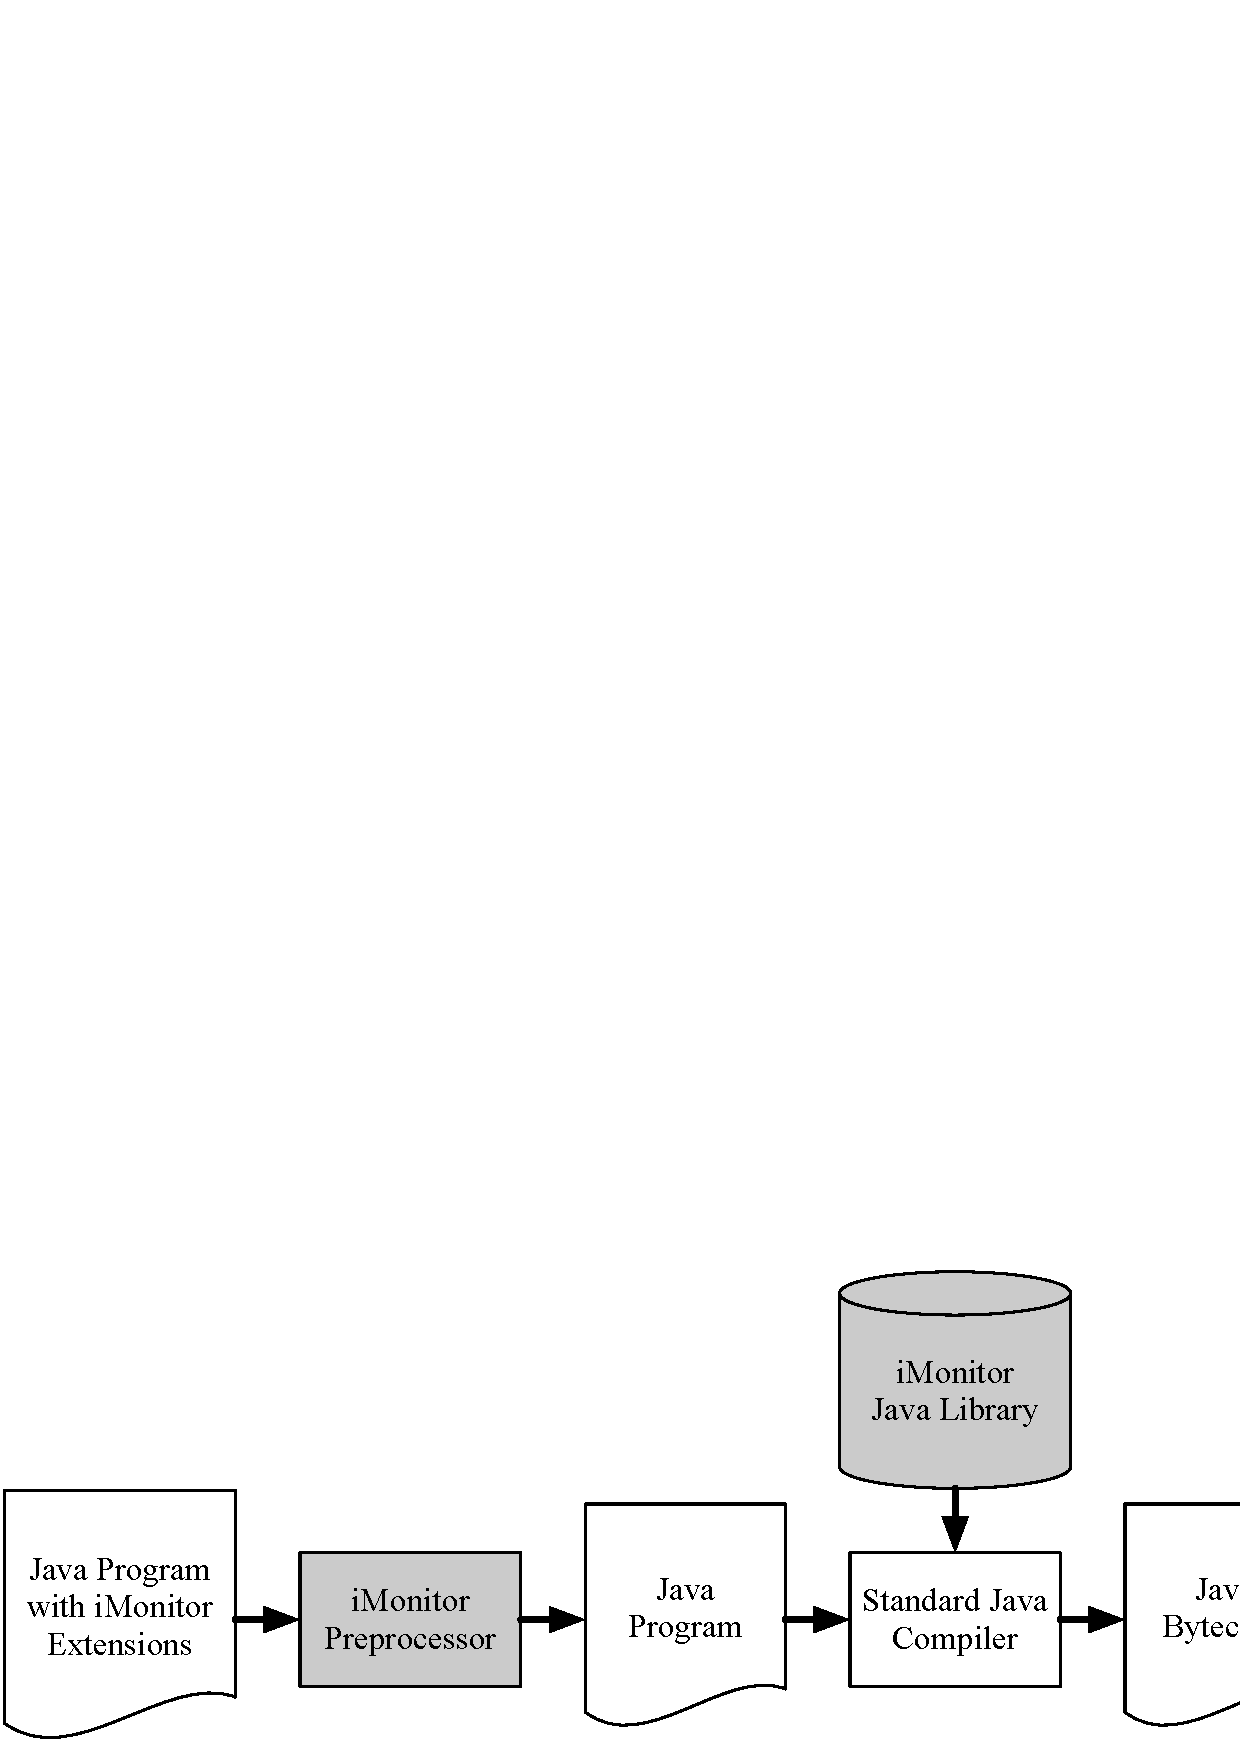
\includegraphics[width=70mm]{fig/flow.png}
  \caption{The framework of iMonitor}
  \label{fig:framework}
\end{figure}



\section{Details of iMonitor Implementation} \label{sec:imp}
The implementation of the implicit-signal monitor in iMonitor involves four 
parts:
\begin{enumerate}
  \item Monitor-constructor: the constructor of the monitor class, including 
    definitions and declarations of additional variables to provide mutual 
    exclusion and synchronization of monitor. 
  \item Monitor-function entry: executed before each member function, 
    involving declarations of additional variables and code to maintain
    mutual exclusion of monitor. 
  \item Monitor-waituntil statement: including declarations of additional
    variables and signal/await statements to implement the waituntil.
  \item Monitor-function leave: executed before the return statement of 
    each member function, involving code to guarantee mutual exclusion and 
    synchronization of monitor. 
\end{enumerate}
%I would like to use Table \ref{tab:constructor_imp},
%\ref{tab:entry_imp}, \ref{tab:waituntilc_imp} and \ref{tab:exit_imp} to sumarize
%the implementations of different kinds of implicit-signal monitors. 



\subsection{Naive}

\begin{SaveVerbatim}{NaiveConstructorImp}
Lock L;
Condition C;
\end{SaveVerbatim}

\begin{SaveVerbatim}{NaiveEntryImp}
lock L 
\end{SaveVerbatim}

\begin{SaveVerbatim}{NaiveWaituntilImp}
if P is false
  signal all C
  do 
    wait C
  while P is false
\end{SaveVerbatim}

\begin{SaveVerbatim}{NaiveExitImp}
signal all C
unlock L
\end{SaveVerbatim}

\begin{SaveVerbatim}{NConditionConstructorImp}
Lock L
List<Predicate, Condition> LIST
foreach global predicate P
  create a pair <P, C>
  add <P, C> to LIST
\end{SaveVerbatim}

\begin{SaveVerbatim}{NConditionWaituntilImp}
if P is a local predicate 
  create a pair <P, C>
  add <P, C> to LIST
 
if P is false 
  foreach <PI, CI> in LIST
    if PI is true
      signal CI
  do 
    wait C
  while P is false

if P is a local predicate 
  remove <P, C> from LIST
\end{SaveVerbatim}

\begin{SaveVerbatim}{NConditionExitImp}
foreach <P, C> in LIST
  if P is true
    signal C

unlock L
\end{SaveVerbatim}


\begin{SaveVerbatim}{MapConditionConstructorImp}
Lock L
Map<Predicate, Condition> MAP
foreach global predicate P
  create a pair <P, C>
  add <P, C> to MAP 
\end{SaveVerbatim}

\begin{SaveVerbatim}{MapConditionWaituntilImp}
if P is a local predicate 
  PE := LocalVariableEvaluation(P)
  if PE is not in MAP
    create a pair <PE, C>
    add <PE, C> to MAP
 
if P is false 
  foreach <PI, CI> in MAP
    if PI is true
      signal CI
  do 
    wait C
  while P is false
\end{SaveVerbatim}

\begin{SaveVerbatim}{MapConditionExitImp}
foreach <PE, C> in MAP
  if PE is true
    signal C

unlock L
\end{SaveVerbatim}


%\begin{table*}
%  \center
%  \begin{tabular}{| l || l | l | }
%    \hline
%    Naive & \BUseVerbatim{NaiveConstructorImp} \\
%                
%    \hline
%    N-Condition & \BUseVerbatim{NConditionConstructorImp} \\
%    \hline
%    Map & \BUseVerbatim{MapConditionConstructorImp} \\
%    \hline
%  \end{tabular}
%  \caption{iMonitor implementation(Contructor)}
%  \label{tab:constructor_imp}
%\end{table*}
%
%\begin{table*}
%  \center
%  \begin{tabular}{| l || l |}
%    \hline
%    Naive & \BUseVerbatim{NaiveEntryImp} \\
%                
%    \hline
%    N-Condition & \BUseVerbatim{NaiveEntryImp} \\
%    \hline
%    Map & \BUseVerbatim{NaiveEntryImp} \\
%    \hline
%  \end{tabular}
%  \caption{iMonitor implementation(Entry)}
%  \label{tab:entry_imp}
%\end{table*}
%
%\begin{table*}
%  \center
%  \begin{tabular}{| l || l |}
%    \hline
%    Naive & \BUseVerbatim{NaiveWaituntilImp} \\
%                
%    \hline
%    N-Condition & \BUseVerbatim{NConditionWaituntilImp} \\
%    \hline
%    Map & \\
%    \hline
%  \end{tabular}
%  \caption{iMonitor implementation(Waituntil C)}
%  \label{tab:waituntilc_imp}
%\end{table*}
%
%\begin{table*}
%  \center
%  \begin{tabular}{| l || l |}
%    \hline
%    Naive & \BUseVerbatim{NaiveExitImp} \\
%                
%    \hline
%    N-Condition & \BUseVerbatim{NConditionExitImp} \\
%    \hline
%    Map & \BUseVerbatim{MapConditionExitImp} \\
%    \hline
%  \end{tabular}
%  \caption{iMonitor implementation(Exit)}
%  \label{tab:exit_imp}
%\end{table*}


In the implementation of naive implicit-signal monitor, one lock variable, 
$L$, is declared for mutual exclusion, which should be acquired in 
the beginning of every member function and released before the return statement.
In addition, one conditional variable, $C$, is declared for 
synchronization, on which the implementation of waituntil depends. In the 
waituntil statement, the predicate expression is checked initially. If the 
expression is false; then all other threads which are waiting on $C$ are 
signaled to reevaluate their predicate expression since the monitor state may 
change. The current thread then is blocked in a loop and reevaluate its 
predicate expression when it is signaled. On the exit of a member function, 
all threads waiting on $C$ are signaled to reevaluate their predicate 
expression since the monitor state may change. Table \ref{tab:imp_naive} 
summarize the implementation of naive implicit-signal monitor. Although 
the naive implicit-signal monitor is easy to implement, it is inefficient. 
When a predicate is evaluated as false or a thread want to leave the monitor, 
all other threads waiting one the same monitor will be awaked and need to 
recheck their conditions.

\begin{table}
    \center
    \begin{tabular}{|l|l|} 
      \hline
      Constructor & \BUseVerbatim{NaiveConstructorImp}\\
      \hline
      Enter & \BUseVerbatim{NaiveEntryImp}\\
      \hline
      Waituntil $P$ & \BUseVerbatim{NaiveWaituntilImp}\\
      \hline
      Exit & \BUseVerbatim{NaiveExitImp} \\
      \hline
    \end{tabular}
    \caption{The naive implicit-signal monitor implementation}
    \label{tab:imp_naive}
\end{table}

\subsection{N-Condition}
Instead of using only one conditional variable for synchronization, the 
N-condition implicit-signal monitor uses multiple conditional variables.
Every predicate in a waituntial statement has an associating conditional variable.
The pair of a predicate assertion and a conditional variable is stored in a shared list, 
$LIST$. For each global predicate, a pair of a predicate and a conditional 
variable is created in the constructor. In the waituntil statement, the type of 
predicate is checked. If the predicate is local predicate, then a corresponding 
conditional variable is created and stored. The predicate expression is then 
checked. If the predicate is false, threads which waits on some true predicates 
are signaled. The current thread then is blocked and recheck 
the predicate expression when it is signaled. After the predicate becomes
true, the pair of predicate and conditional variable is removed from the 
$LIST$ if the predicate ls local predicate. When a thread finishes jobs and wants
to leave the monitor, the list of predicates are checked. Thread which wait 
on a true predicate are signaled. Table \ref{tab:imp_n_cond} summarized the 
implementation. Note that, only threads waiting on the true predicates are
signaled. Therefore, the number
of unnecessary signals and predicate checking is reduced. Moreover, it prevents programers form abusing
signalAll statement in explicit-signal monitor. However,  when a thread 
executes the waituntil statement, 
a conditional variable is created for a local predicate. It is extremely 
expensive when waituntil statements with local predicates are executed many
times.
% remove signal all 

\begin{table}
    \center
    \begin{tabular}{|l|l|} 
      \hline
      Constructor & \BUseVerbatim{NConditionConstructorImp}\\
      \hline
      Enter & \BUseVerbatim{NaiveEntryImp}\\
      \hline
      Waituntil $P$ & \BUseVerbatim{NConditionWaituntilImp}\\
      \hline
      Exit & \BUseVerbatim{NConditionExitImp} \\
      \hline
    \end{tabular}
    \caption{The N-condition implicit-signal monitor implementation}
    \label{tab:imp_n_cond}
\end{table}

\subsection{Map-Condition}
The map-condition predicate uses the data structure map to store pairs of 
predicate and conditional variables. A predicate and a corresponding conditional
variable are treated as key and value respectively. For every global predicate, 
a corresponding conditional variable is created and the pair of a predicate and a
conditional variable is added to the map in the constructor. For every local 
predicate, the globalization has been applied to the local 
predicate. Every local variable is replaced in the local predicate by its value
at this point. The globalization does not affect on the results of 
predicate evaluations since other threads cannot change the value of local 
variables but only global variables. After applying globalization to
the local predicate, a new predicate with only global variable is derived. 
If the predicate has not been added to the shared map, then the new 
predicated is added to the map with a corresponding conditional variable.
Otherwise, the corresponding conditional variable can be found by searching the
predicate in the map. Hence, the number of creating and removing conditional
variables has been reduced. 


\begin{table}
    \center
    \begin{tabular}{|l|l|} 
      \hline
      Constructor & \BUseVerbatim{MapConditionConstructorImp}\\
      \hline
      Enter & \BUseVerbatim{NaiveEntryImp}\\
      \hline
      Waituntil $P$ & \BUseVerbatim{MapConditionWaituntilImp}\\
      \hline
      Exit & \BUseVerbatim{MapConditionExitImp} \\
      \hline
    \end{tabular}
    \caption{The map-condition implicit-signal monitor implementation}
    \label{tab:imp_map_cond}
\end{table}

\section{Evaluations} \label{sec:eval}
To evaluate the performance of iMonitor, both implicit- and explicit-monitor 
solutions for different problems were implemented. We would like to evaluate the
runtime of different approaches. All of the experiments were conducted on a 
machine with 16 Intel(R) Xeon(R) X5560 CPUs and 64 GBs memory.



\subsection{Bounded-Buffer Problem}
\subsection{Reader/Writer Problem}
\subsection{Dining Philosophers  Problem}
%The dining philosophers problem is often used in computer science to describe 
%the synchronization issues. There are N philosophers siting around at a table 
%with a dish in front of them and a chopstick in between each philosopher. A 
%philosopher only think or eat. A philosopher needs to pick two chopsticks at the
%same time for eating and he does not put down a chopstick until he finishes 
%eating. If the chopstick is hold by another philosopher, then the philosopher 
%who want to eat must wait. In addition, a philosopher cannot eat forever, which
%means he will put down chopstick eventually. Every philosopher must be able to
%eat eventually if he is hungry. Figure 3. illustrate the experimental results
%of the dining philosophers problem. The x-axis depicts the runtime and the 
%y-axis describes the number of philosophers. As can be seen, three approaches 
%has the similar results. The implementations of Naive and N-condition are as 
%efficient as the implementation of explicit signal monitor. 
%
\subsection{Access Patterns}

%\section{Discussions}
%\subsection{Comparision between different implementations}
%\subsection{Practical Issues} Need a big project to demonstrate 


\section{Conclusions} \label{sec:conclu}

\appendix
\section{Appendix Title}

This is the text of the appendix, if you need one.

\acks

Acknowledgments, if needed.

% We recommend abbrvnat bibliography style.

\bibliographystyle{abbrvnat}

% The bibliography should be embedded for final submission.

\begin{thebibliography}{}
    \softraggedright

  \bibitem {bh05}
    P. A. Buhr and A. S. Harji. Implicit-Signal Monitors. ACM Transactions on 
    Programming Languages and Systems ACM, 27(6):1270-1343, Nov. 2005.

  \bibitem {hoa74}
     C. A. R. Hoare. Monitors: an operating system structuring concept. Commun. 
     ACM 17, 10(Oct. 1974), 549-557.

\end{thebibliography}

\end{document}
